\documentclass[12pt]{article}
\usepackage{note}

\title{W decay to massive quarks}
\author{Ivan Pogrebnyak}
\date{\today}

\begin{document}
\maketitle

\begin{figure}[H]
  \centering
  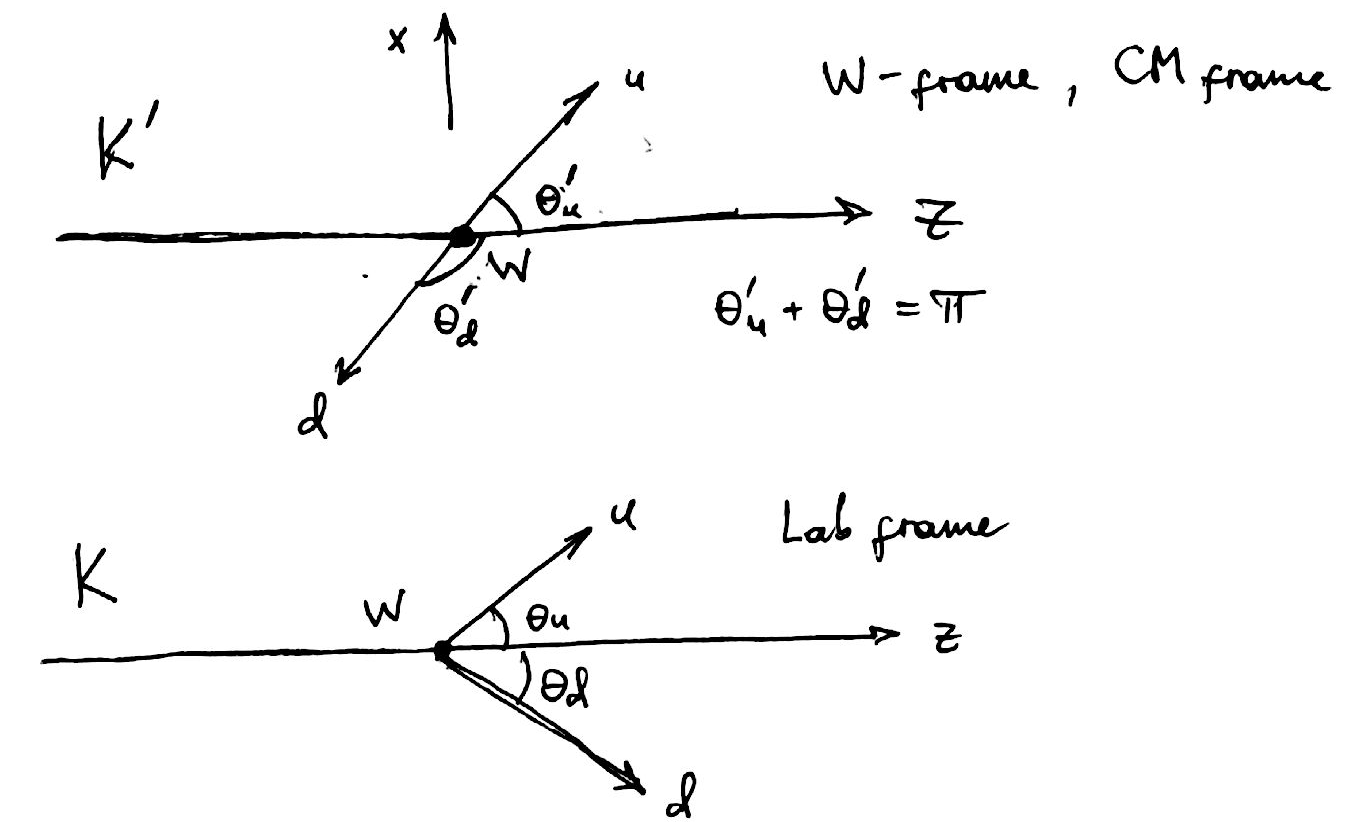
\includegraphics[width=0.65\textwidth]{fig/fig.png}
\end{figure}

{\bf Boost from rest frame:}
\begin{equation}
  P = \Lambda P' \quad \Leftrightarrow \quad
%
  \begin{pmatrix} E\\0\\0\\p \end{pmatrix} =
  \begin{pmatrix}
    \gamma & 0 & 0 & \gamma\beta \\
    0 & 1 & 0 & 0 \\
    0 & 0 & 1 & 0 \\
    \gamma\beta & 0 & 0 & \gamma \\
  \end{pmatrix}
  \begin{pmatrix} m\\0\\0\\0 \end{pmatrix}
  \quad \Rightarrow \quad
%
  \left\{\begin{array}{l}
    E = \gamma m \\
    p = \gamma\beta m
  \end{array}\right.
\end{equation}
%
\begin{equation}
  \gamma = \frac{E}{m}, \quad
  \gamma\beta = \frac{p}{m}, \quad
  \beta = \frac{p}{E}
\end{equation}

%%%%%%%%%%%%%%%%%%%%%%%%%%%%%%%%%%%%%%%%%%%%%%%%%%%%%%%%%%%%%%%%%%%%%%%%%%

{\bf In the lab frame, $K$:}
\begin{equation}\label{eq:pLab}
  P_W = (E_W,0,0,p_W), \quad
  P_u = (E_u,p_u\sin\theta_u,0,p_u\cos\theta_u), \quad
  P_d = (E_d,-p_d\sin\theta_d,0,p_d\cos\theta_d)
\end{equation}
%
By conservation of momentum,
\begin{equation}\label{eq:consLab}
  \left\{\begin{array}{l}
    E_W = E_u + E_d, \\
    p_u\sin\theta_u = p_d\sin\theta_d, \\
    p_W = p_u\cos\theta_u + p_d\cos\theta_d.
  \end{array}\right.
  \quad
  \begin{array}{l}
    +\begin{array}{l}
      p_d^2\cos^2\theta_d = p_W^2 + p_u^2\cos^2\theta_u - 2p_Wp_u\cos\theta_u \\
      p_d^2\sin^2\theta_d = p_u^2\sin^2\theta_u
    \end{array} \\
    \hline
    \hspace{17mm} p_d^2 = p_W^2 + p_u^2 - 2p_Wp_u\cos\theta_u
  \end{array}
\end{equation}
%
\begin{equation}\label{eq:cos}
  \therefore
  \cos\theta_u = \frac{p_W^2 + p_u^2 - p_d^2}{2p_Wp_u}
\end{equation}

%%%%%%%%%%%%%%%%%%%%%%%%%%%%%%%%%%%%%%%%%%%%%%%%%%%%%%%%%%%%%%%%%%%%%%%%%%

{\bf In the CM frame, $K'$:}
\begin{equation}\label{eq:pCM}
  P'_W = (m_W,0,0,0), \quad
  P'_u = (E'_u,p'_u\sin\theta'_u,0,p'_u\cos\theta'_u), \quad
  P'_d = (E'_d,-p'_d\sin\theta'_d,0,p'_d\cos\theta'_d).
\end{equation}
%
By conservation of momentum,
\begin{equation}\label{eq:consCM}
  \left\{\begin{array}{l}
    m_W = E'_u + E'_d, \\
    p'_u\sin\theta'_u = p'_d\sin\theta'_d, \\
    p'_u\cos\theta'_u =-p'_d\cos\theta'_d.
  \end{array}\right.
\end{equation}
%
By the sum of squares of the last two equalities in \eq{consCM}, using
$\sin^2\theta + \cos^2\theta = 1$,
\begin{equation}\label{eq:eqmom}
  p'_q = p'_{u} = p'_{d}, \quad
  \sin\theta'_d =  \sin\theta'_u, \quad
  \cos\theta'_d = -\cos\theta'_u,
\end{equation}
i.e. the momenta of the final state quarks in the $W$-frame are equal and oposite.

By the first equality in \eq{consCM}, using $E^{2} = p^{2}+m^{2}$,
\begin{equation}
  m_W^2 = {E'_u}^{2} + {E'_d}^{2} + 2E'_uE'_d
  = {p'_u}^2 + {m_u}^2 + {p'_d}^2 + {m_d}^2 + 2\sqrt{({p'_u}^2 + {m_u}^2) ({p'_d}^2 + {m_d}^2)}
\end{equation}
%
\def\massroot{\sqrt{ m_W^4 - 2m_W^2(m_u^2+m_d^2) + (m_u^2-m_d^2)^2 }}
Using \eq{eqmom}, it can be shown that
\begin{equation}
  p'_q = \frac{\massroot}{2m_W},
\end{equation}
and
\begin{equation}
  E'_u = \sqrt{{p'_u}^2 + m_u^2} = \frac{m_W^2 + m_u^2 - m_d^2}{2m_W}.
\end{equation}
%
For massless quarks, we obtain the expected result
\begin{equation}
  \lim_{m_q\rightarrow 0} p'_q = \lim_{m_q\rightarrow 0} E'_q = \frac{m_W}{2}.
\end{equation}

%The quark 4-momentum can thus be written as,
%\begin{equation}\label{eq:pCM2}
%  P'_q = \left(\sqrt{{p'_q}^2+m_q^2},\ p'_q\sin\theta'_q,\ 0,\ p'_q\cos\theta'_q\right).
%\end{equation}

%%%%%%%%%%%%%%%%%%%%%%%%%%%%%%%%%%%%%%%%%%%%%%%%%%%%%%%%%%%%%%%%%%%%%%%%%%

{\bf Applying Lorentz transformation:}
%
\begin{align}
  \begin{pmatrix}
    E_q \\
    \pm p_q\sin\theta_q \\
    0 \\
    p_q\cos\theta_q
  \end{pmatrix} &=
  P_q = \Lambda P'_q =
  \begin{pmatrix}
    \gamma & 0 & 0 & \gamma\beta \\
    0 & 1 & 0 & 0 \\
    0 & 0 & 1 & 0 \\
    \gamma\beta & 0 & 0 & \gamma \\
  \end{pmatrix}
  \begin{pmatrix}
    E'_q \\
    \pm p'_q\sin\theta'_u \\
    0 \\
    \pm p'_q\cos\theta'_u
  \end{pmatrix}
  =
  \begin{pmatrix}
    \gamma E'_q \pm \gamma\beta p'_q\cos\theta'_u \\
    \pm p'_q\sin\theta'_u \\
    0 \\
    \gamma\beta E'_q \pm \gamma p'_q\cos\theta'_u
  \end{pmatrix}
\end{align}
%
\begin{equation}
  \therefore
  p_q^2 = \gamma^2 (E'_q \pm \beta p'_q\cos\theta'_u)^2 - m_q^2
\end{equation}
%
Substituting into \eq{cos},
\begin{align}
  \cos\theta_u = \frac{p_W^2 + p_u^2 - p_d^2}{2p_Wp_u}, \quad
  \cos\theta_d = \frac{p_W^2 + p_d^2 - p_u^2}{2p_Wp_d}
\end{align}
%
\begin{equation}
  \tan\theta = \frac{\sin\theta}{\cos\theta}
  = \frac{\sqrt{1-\cos^2\theta}}{\cos\theta}
\end{equation}
%

\begin{equation}\label{eq:result}
  \boxed{
    \theta_\mathrm{opening}
    = \tan^{-1}(\tan\theta_u) + \tan^{-1}(\tan\theta_d)
  }
\end{equation}

%\begin{figure}[H]
%  \centering
%  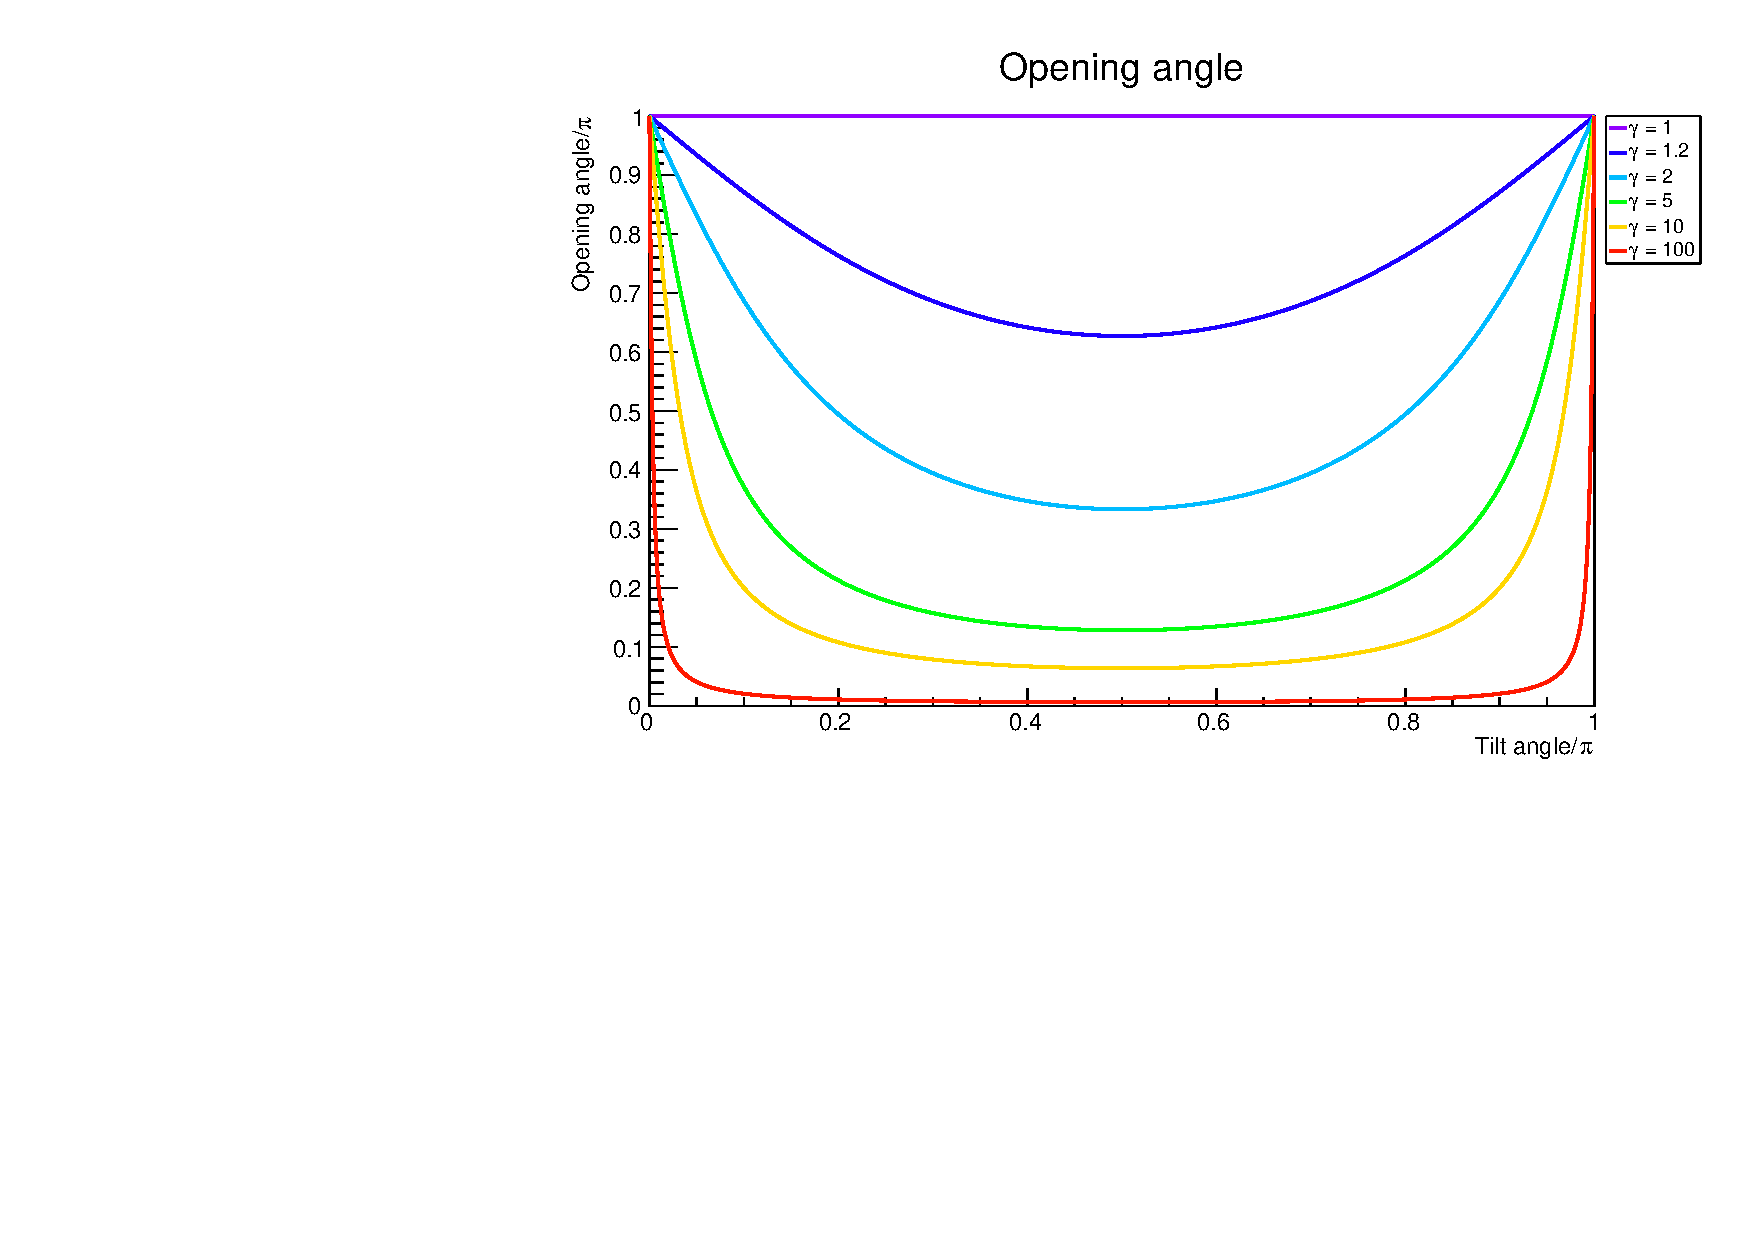
\includegraphics[width=\textwidth]{fig/opening_angle.pdf}
%\end{figure}

\end{document}
